\chapter{Case Study}\label{ch:case study}

\newcommand{\mysubparagraph}[1]{\subparagraph{#1}\mbox{}\\}

\section{Problem}


\subsection{Research Questions}
\begin{enumerate}
\item In what ways do the tools correlate?
\item How much complete are the tools in measuring agility?
\item Can the tools be combined in a way so that they can produce a more complete approach on measuring agility?
\end{enumerate}

\section{Method}

\subsection{Case Study Design}

\subsection{Case and Subjects Selection}

\subsection{Observations}
Company F \footnote{F is the first letter of the company's name} was willing to participate in this case study in order to measure how agile are its teams. With previous work experience in this company I had an insight of how the teams work and what each of them wants to achieve each one of them. Nevertheless I spent 3 months working closely with the teams almost daily for the needs of the master thesis.

\subsection{Company F}
Company F is a United States company which acts in the POS \footnote{Point Of Sales} area. With the development of some new products the company had a 300\% increase in the size of the development and QA departments resulting in the need for organizing better the development and release processes. In addition the increasing requests of new features in the company's systems requires a more efficient way in delivering them to the customers and also maintaining the quality of the products.

\subsection{Methodology F}
In general, company F does not follow a specific agile methodology, but rather a tailored mix of the most famous one which suits the needs of each team. Methodology F, as we can name it, embraces the practices displayed in Table~\ref{table:methodologyF_practices} from the various agile methodologies, some of the them in bigger and some of them in a smaller extent. For identifying these methodologies the analysis made by \cite{koch2005agile} was used. The results were verified by the agile coach.

\begin{table}
\caption{Practices embraced in methodology F}
\begin{tabular}{| p{2cm} | p{13cm}|}
    \hline
     \textbf{Method} & \textbf{Practice} \\ \hline
     \textbf{XP}  & \begin{inparaenum} [a\upshape)]
     				\item Small Releases \item Simple design \item Refactoring \item Collective ownership \item Continuous integration \item 40-hour week \item Coding standards
					\end{inparaenum}      \\ \hline
     \textbf{FDD}  & \begin{inparaenum} [a\upshape)]  \item Developing by feature \item Feature teams \item Regular build schedule \item Inspections \item Configuration management
     				  \end{inparaenum}\\ \hline
     \textbf{Lean} & \begin{inparaenum} [a\upshape)] \item Empower the team \item Build Integrity In \item Amplify learning \item Eliminate waste
     				 \end{inparaenum} \\ \hline
\end{tabular}
\label{table:methodologyF_practices}
\end{table}


\subsection{Teams}
There are four development teams, each for a product of the company. Some of the teams have mixed members of developers and testers. In the Tables~\ref{table:teamA}, \ref{table:teamB}, \ref{table:teamC}, \ref{table:teamD}, one can see the structure of the teams. \\

\begin{table}
  \RawFloats
 \begin{minipage}[b]{0.5\textwidth}
  \centering
    \caption{Team A - Profile} %Mobile
  \begin{tabular}{| p{3cm} | p{3cm}|}
    \hline
     \textbf{Team Size} & 7 \\ \hline
     \textbf{Roles}  & \begin{tabular}{@{}l@{}}Team Leader (1) \\ Developers (4) \\ Testers (3) \end{tabular} \\ \hline
     \textbf{Development Process}  & Method A \\ \hline
     \textbf{Area} & Mobile \\ \hline
     \textbf{Tools used}  & \begin{tabular}{@{}l@{}}Perforce \\ Titanium \end{tabular}  \\ \hline
     \textbf{Iteration length}  & 2-3 weeks \\ \hline
  \end{tabular}
  \label{table:teamA}
 \end{minipage} %
%
 \begin{minipage}[b]{.5\textwidth}
  \centering
    \caption{Team B - Profile} %Marketing
  \begin{tabular}{| p{3cm} | p{3cm}|}
    \hline
     \textbf{Team Size} & 8 \\ \hline
     \textbf{Roles}  & \begin{tabular}{@{}l@{}}Team Leader (1) \\ Developers (5) \\ Testers (2) \end{tabular} \\ \hline
     \textbf{Development Process}  & Method B \\ \hline
     \textbf{Area} & Java \\ \hline
     \textbf{Tools used}  & \begin{tabular}{@{}l@{}}Perforce \\ Eclipse IDE \end{tabular} \\ \hline
     \textbf{Iteration length}  & 2-3 weeks \\ \hline
  \end{tabular}
  \label{table:teamB}
  \end{minipage} %
  
  \vspace{10 mm}
%
 \begin{minipage}[b]{.5\textwidth}
  \centering
    \caption{Team C - Profile} %Info
  \begin{tabular}{| p{3cm} | p{3cm}|}
    \hline
     \textbf{Team Size} & 3 \\ \hline
     \textbf{Roles}  & \begin{tabular}{@{}l@{}}Team Leader (1) \\ Developers (1) \\ Testers (1) \end{tabular} \\ \hline
     \textbf{Development Process}  & Method C \\ \hline
     \textbf{Area} & Java \\ \hline
     \textbf{Tools used}  & \begin{tabular}{@{}l@{}}Perforce \\ Eclipse IDE \end{tabular}  \\ \hline
     \textbf{Iteration length}  & 4-5 weeks \\ \hline
  \end{tabular}
  \label{table:teamC}
\end{minipage}%
%
 \begin{minipage}[b]{.5\textwidth}
  \centering
    \caption{Team D - Profile} %POS
  \begin{tabular}{| p{3cm} | p{3cm}|}
    \hline
     \textbf{Team Size} & 17 \\ \hline
     \textbf{Roles}  & \begin{tabular}{@{}l@{}}Team Leader (1) \\ Developers (9) \\ Testers (7) \end{tabular} \\ \hline
     \textbf{Development Process}  & Method D \\ \hline
     \textbf{Area} & Java \\ \hline
     \textbf{Tools used}  & \begin{tabular}{@{}l@{}}Perforce \\ Eclipse IDE \end{tabular} \\ \hline
     \textbf{Iteration length}  & 2-4 weeks \\ \hline
  \end{tabular}
  \label{table:teamD}
  \end{minipage}
\end{table}


%analyze more what each team does

\subsection{Products}
Company F has developed a few products which belong in the following four areas 
\begin{inparaenum} [a\upshape)]
\item desktop
\item mobile
\item cloud
\item platforms.
\end{inparaenum}
The names given are respectives to the name of the teams that develop them.

\begin{itemize}
\item Product A - A series of three mobile applications which offer services to stores or customers of stores.
\item Product B - It is a cloud application which offers services to product A and product D. The web functionality of product C is limited.
\item Product C - It is a platform used only by the company's employees. It supports services though which are necessary for product D.
\item Product D - It is the main product of the company which is mostly used. The rest of the products were developed in order to support it and expand its functionalities.

\end{itemize}

\section{OPS}

\subsection{Introduction}
In order to measure the adequacy, the capability and the effectiveness of methodology F, the described method by \citet{sventha_dissertation} was followed.

\subsection{Adequacy Assessment}
\label{subsec:adequacy_analysis}

In order to assess the adequacy of methodology F a top-down traversal was used as it can be seen in Figure~\ref{ops_core}. For the analysis of each objective, principle and strategy the analysis of agile methodologies was followed based on \citet{koch2005agile}.

Initially the objectives fulfilled by methodology F were identified. As one can see in Figure~\ref{fig:companyF_objectives} all five objectives instructed by the OPS Framework are followed.

\begin{figure}[H]
\centerline{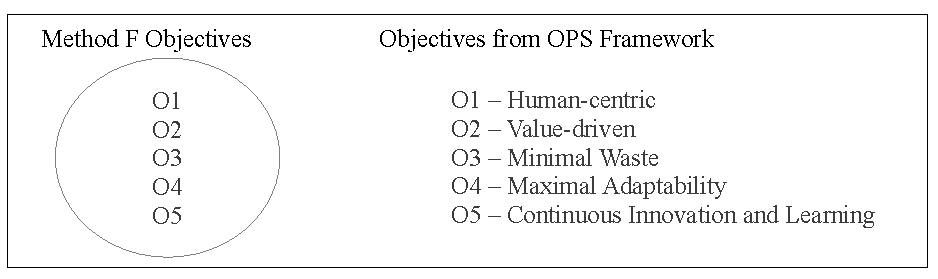
\includegraphics[scale=0.9]{include/case_study/fig/companyF_objectives.pdf}}
\caption{Objectives identified in methodology F} 
\label{fig:companyF_objectives}
\end{figure}

Based on the objectives and following the linkages from them, the principles were identified. As one can see in Figure~\ref{fig:companyF_objectives} methodology F does not follow the ``Frequent Reflection and Improvement" principle because the organization rarely does it re-examine the development process in order to improve it. %maybe justify why!
It is worth mentioning that the ``Empowering teams of Motivated Individuals" principle is not entirely followed either, but it differs among the teams. Every team is built with motivated individuals, some to a more and some to a lesser extent. 

\begin{figure}[H]
\centerline{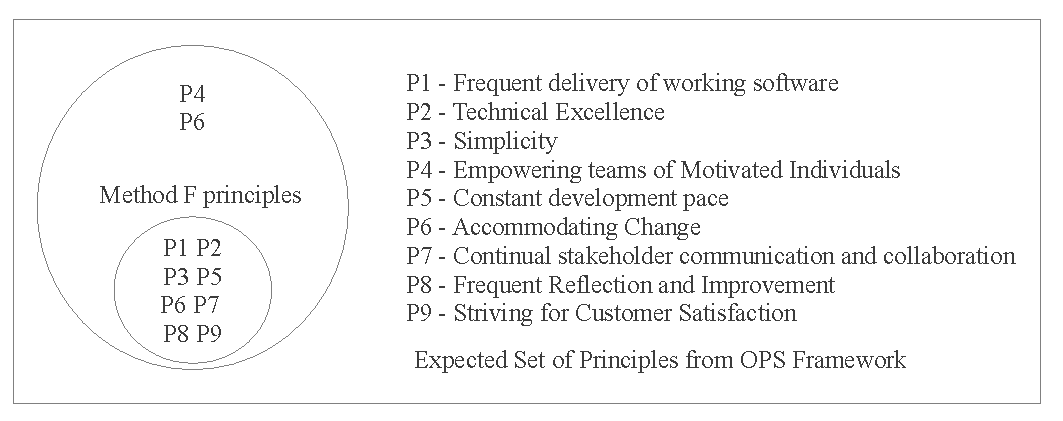
\includegraphics[scale=0.9]{include/case_study/fig/companyF_principles.pdf}}
\caption{Principles identified in methodology F} 
\label{fig:companyF_principles}
\end{figure}

Following the linkages from the principles the strategies for implementing them were identified. As it can be seen in Figure~\ref{fig:companyF_strategies} methodology F does not support 

\begin{itemize}
\item \textbf{Continuous feedback} - The organization does not have a defined process for getting a feedback from the customers of the company. From time to time the managers of the various departments of the company have personal conversations with the customers. If any issue arises, then they inform the development and QA departments in order to identify the problem and fix it.
\item \textbf{Test-first development} - None of the team members writes tests before starting coding.
\item \textbf{Constant velocity} - The organization does not measure the velocity of the teams. In general the pace of development and integration and deployment is based on the needs of the customers and the capability of the developer. No one has to finish a specific amount of work in each iteration. What is only wanted, is the functionality to be delivered when it is scheduled.
\item \textbf{Retrospection} - Although there is a tendency to change this, the teams do not have a process for retrospection. The team members unconsciously consider that they are doing fine, unless a team leader or the manager of the department tells them the opposite.
\end{itemize}

\begin{figure}[H]
\centerline{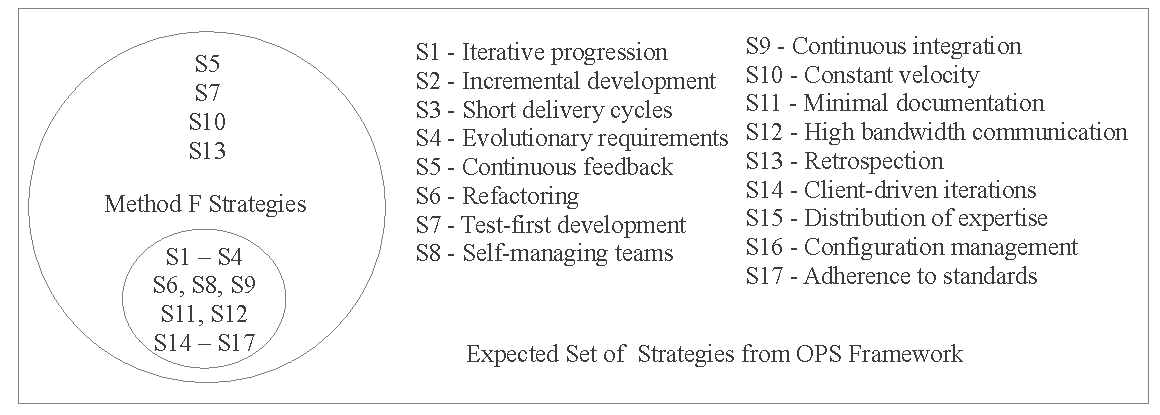
\includegraphics[scale=0.9]{include/case_study/fig/companyF_strategies.pdf}}
\caption{Strategies identified in methodology F} 
\label{fig:companyF_strategies}
\end{figure}

%Analyze more the adequacy
Reflecting on the above analysis, we see that methodology F lacks four strategies which are important for its improvement. Without retrospection the team members do not always identify and discuss their mistakes, while without a well defined process for continuous feedback any issues that might arise may go unnoticed for quite some time. In total, methodology F is missing four strategies out of seventeen which is a lot. As a result the adequacy of methodology F is questionnable.

\subsection{Capability and Effectiveness Assessement}
In order to assess the capability and effectiveness of methodology F a bottom-up traversal was used as it can be seen in Figure~\ref{ops_core}. Based on the adequacy analysis performed in subsection~\ref{subsec:adequacy_analysis} the assessment of the capability and effectiveness started from the strategies and following the linkages moved to the principles and then to the objectives. 

As an observer of the teams I filled in the questions from the capability and effectiveness hierarchy. The scales used were the ones proposed by \citet{sventha_dissertation}. A ternary scale for the capability and a scale between 1-5 for the effectiveness (see Table~\ref{table:capability_scale} and  Table~\ref{table:effectiveness_scale} respectively). For the interpration of the scores for both the capability and effectiveness the scale in Table~\ref{table:scale_for_final_scores} was used. All the questions answered can be seen in~\nameref{sec:capability_hierarchy} and~\nameref{sec:effectiveness_hierarchy} Appendices. \\

\begin{table}
\RawFloats %allows to have captions in all of the tables
 \begin{minipage}{.3\textwidth}
  \caption{Scale for Capability}
  \label{table:capability_scale}
  \begin{tabular}{| c | c |}
 \hline
 \textbf{Answer} & \textbf{Score} \\ \hline
 Yes/Fully & 5 \\ \hline
 Partially & 3 \\ \hline
 No/Marginally & 1 \\ \hline 
 \end{tabular}
 \end{minipage}%
%
 \begin{minipage}{.35\textwidth}
  \centering
 \caption{Scale for Effectiveness}
 \label{table:effectiveness_scale}
  \begin{tabular}{| c | c |}
 \hline
 \textbf{Answer} & \textbf{Score} \\ \hline
 Maximally & 5 \\ \hline
 Considerably & 5 \\ \hline
 Moderately & 3 \\ \hline
 Somewhat & 2 \\ \hline
 Marginally & 1 \\ \hline 
 \end{tabular}
 \end{minipage}%
 %
 \begin{minipage}{.35\textwidth}
  \caption{Scale for interpreting final scores}
  \label{table:scale_for_final_scores}
  \centering
 \begin{tabular}{| c | c |}
 \hline
 \textbf{Score Range} & \textbf{Interpretation} \\ \hline
 4.5 - 5.0 & Maximal \\ \hline
 3.5 - 4.4 & Considerable \\ \hline
 2.5 - 3.4 & Moderate \\ \hline
 1.5 - 2.4 & Somewhat \\ \hline
 1 - 1.4 & Marginal \\ \hline 
 \end{tabular}
 \end{minipage}%
\end{table}



\subsubsection{General remarks about the teams}

\subsubsection{Team A Assessement}
\begin{tabular}{| p{6cm} | p{6cm}|}
\hline
\textbf{Capability:} 2.3 - Somewhat & \textbf{Effectiveness:} 2.3 - Somewhat \\ \hline
\end{tabular} \\

Team A is a team with seven members. One team leader, four developers and three testers. The product is a series of mobile applications either for the stores, or the customers of the stores.

\paragraph{Capability Analysis}

\mysubparagraph{Strategies} 
The team differs from the rest in the \textit{adherence to standards} strategy. This is because there are no specified techniques yet to identify the features for the applications. Since they are fairly new the team members are still in the process of working it out. In addition some of the team members do not follow the coding standards of the company resulting in badly written code which has been refactored already twice because of this. As far as the \textit{evolutionary requirements} strategy is concerned, as it was mentioned above, the applications are failry new and the team is still working on improving the process of identifying and modifying the requirements.

\mysubparagraph{Principles}
The team is in accordance with the rest.

\mysubparagraph{Objectives} 
The team is in accordance with the rest.

\paragraph{Effectiveness Analysis}

\mysubparagraph{Strategies} 
The \textit{high bandwidth communcation} has the lowest value, mostly because the developers work on different applications and rarely have to communicate with each other, unless they need some help.

\mysubparagraph{Principles}
The team is in accordance with the rest.

\mysubparagraph{Objectives} 
The team is in accordance with the rest.


\subsubsection{Team B Assessement}
\begin{tabular}{| p{6cm} | p{6cm}|}
\hline
\textbf{Capability:} 2.6 - Moderate & \textbf{Effectiveness:} 2.4 - Somewhat \\ \hline
\end{tabular} \\

Team B is a team with an average size. It consists of eight members. One team  leader, five developers and two testers. The product provides services which are used by product A and product C. The application itself is in Amazon Web Services (AWS).

\paragraph{Capability Analysis}

\mysubparagraph{Strategies} 
The team differs from the rest in the \textit{self managing teams} strategy since this team always consisted of the most motivated but also valualble technically developers. Since the decisions for the new features are taken 85\% from the team itself, the client driven iterations and incremental development are high.

\mysubparagraph{Principles}
The team has the highest value for the empowering teams of motivated individuals principle for the reason that was mentioned right above. In addition since the customer are the members themselves the striving for customer satisfaction principle has the highest value.

\mysubparagraph{Objectives} 
The team has the highest values in all the objectives. This is because......

\paragraph{Effectiveness Analysis}

\mysubparagraph{Strategies} 
The team differs in the client driven iterations strategy for the reasons mentioned above.

\mysubparagraph{Principles}
The team differs in theempowering teams of motivated individuals principle for the reasons mentioned above.

\mysubparagraph{Objectives} 
The team is in accordance with the rest.

\subsubsection{Team C Assessement}
\begin{tabular}{| p{6cm} | p{6cm}|}
\hline
\textbf{Capability:} 2.3 - Somewhat & \textbf{Effectiveness:} 2.5 - Moderate \\ \hline
\end{tabular} \\

Team C is the smallest team of the company, with only three team members. One team leader, one developer and one tester. The product developed is only internally used by the company iteself, nevertheless, it is of great importance since without it the non developer and tester employees would not be able to work. In addition, it is needed by the rest products to properly work.

\paragraph{Capability Analysis}

\mysubparagraph{Strategies} 
The team differs from the rest in the \textit{client driven iterations}, the \textit{short delivery cycles} and the \textit{minimal documentation} strategies. This is the only team with such a high score for the client driven iteration. Since the product is only used by the employees of the company then the identification and priortization of the features is done constantly and immediately. As far as the short delivery cycles, since there are no ``external" customers waiting for it, the releases cycle depends only on the features being worked. If nothing important is under development, there is no rush to release it. Finally this is the product with the least documentation maintained, for the same reasons that the other two aformentioned strategies differ.

\mysubparagraph{Principles}
The team is in accordance with the rest.

\mysubparagraph{Objectives} 
The team is in accordance with the rest.

\paragraph{Effectiveness Analysis}

\mysubparagraph{Strategies}
The team differs follows the same trend with team D for the continuous integration. This is because there are unit test suites and no automated build environment. As far as the high-bandwidth communication is concerned, the team has the highest score, due to the fact the the size of the team is minimal and all the communication is fast and easy. The customer satisfaction is high as well, since ``the product is built right", reinforcing not only this strategy, but also the client-driven iteration one.

\mysubparagraph{Principles}
As it was mentioned before, due to the team size the individuals are extremely motivated and feel responsible for the product.

\mysubparagraph{Objectives}
The team is in accordance with the rest.


\subsubsection{Team D Assessement}
\begin{tabular}{| p{6cm} | p{6cm}|}
\hline
\textbf{Capability:} 2.4 - Somewhat & \textbf{Effectiveness:} 2.2 - Somewhat \\ \hline
\end{tabular} \\

Team D is the biggest team of the company. It consists of 17 members. One team leader, nine developers and seven testers. The product created is the main product of the company and thus it has many needs for people working on it. 

\paragraph{Capability Analysis}

\mysubparagraph{Strategies} 
The team is in accordance with the rest.

\mysubparagraph{Principles}
The team is in accordance with the rest.

\mysubparagraph{Objectives} 
The team is in accordance with the rest.

\paragraph{Effectiveness Analysis}

\mysubparagraph{Strategies} 
This differs from the rest in the \textit{distribution of expertise}, since it is the biggest team the average of the team member's capabilities is low and as result the score for this strategy is the lowest as well.

\mysubparagraph{Principles}
The team is in accordance with the rest.

\mysubparagraph{Objectives} 
The team is in accordance with the rest.


\begin{figure}[H]
\centerline{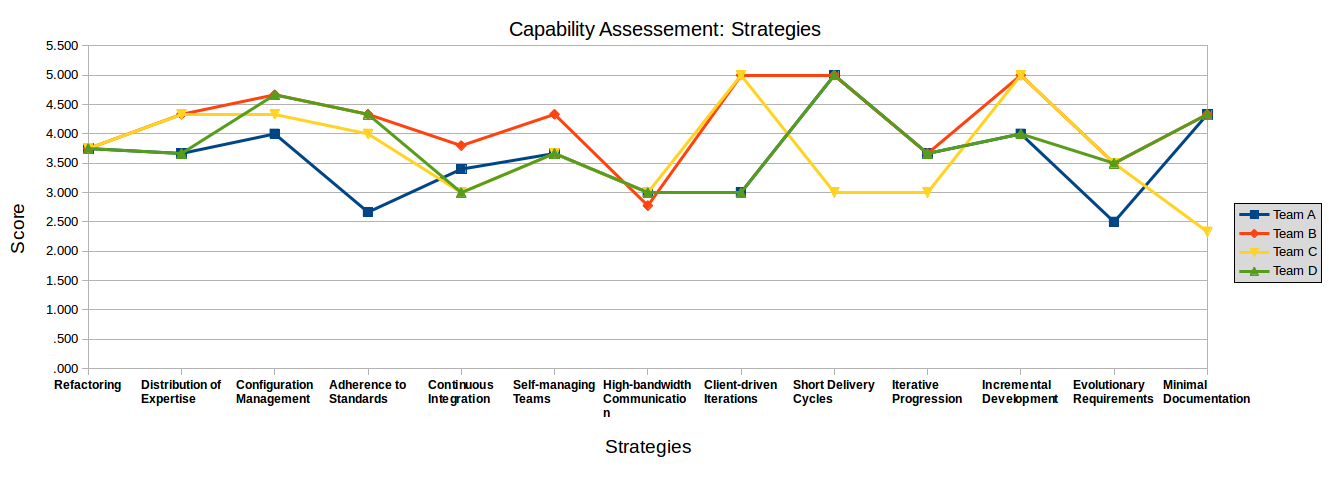
\includegraphics[scale=0.55]{include/case_study/fig/team_capability_strategies.png}}
\caption{Capability - Strategies level} 
\label{fig:team_capability_strategies}
\end{figure}

\begin{figure}[H]
\centerline{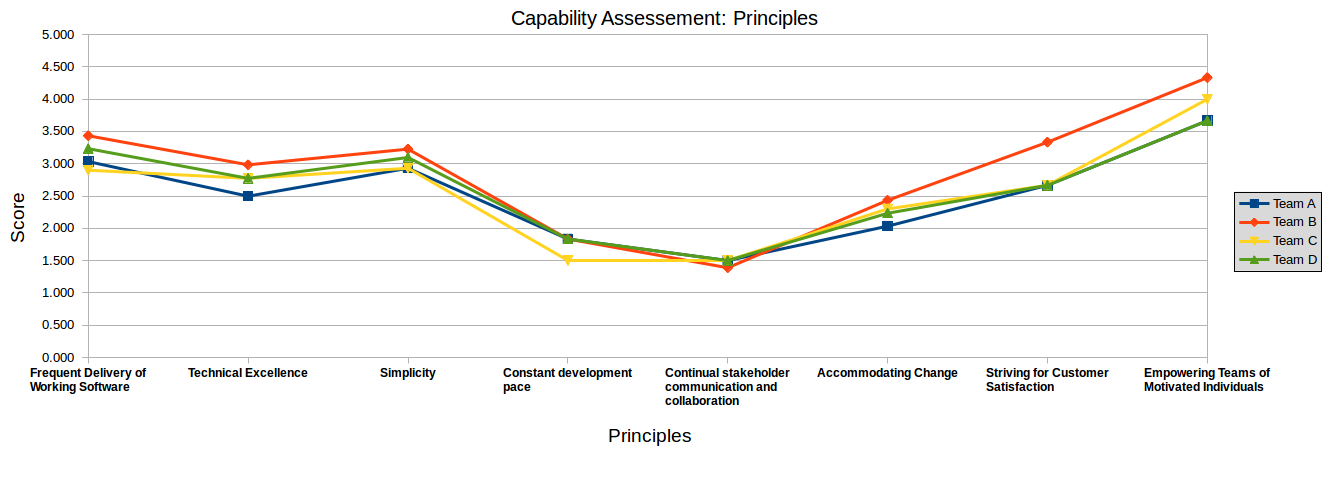
\includegraphics[scale=0.55]{include/case_study/fig/team_capability_principles.png}}
\caption{Capability - Principles level} 
\label{fig:team_capability_principles}
\end{figure}

\begin{figure}[H]
\centerline{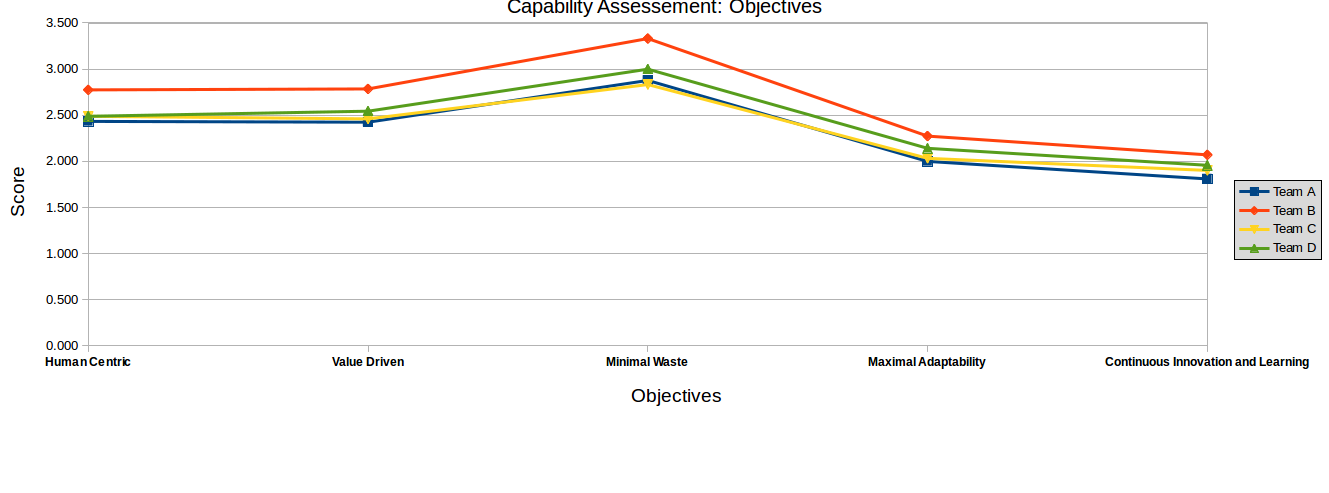
\includegraphics[scale=0.55]{include/case_study/fig/team_capability_objectives.png}}
\caption{Capability - Objectives level} 
\label{fig:team_capability_objectives}
\end{figure}

\begin{figure}[H]
\centerline{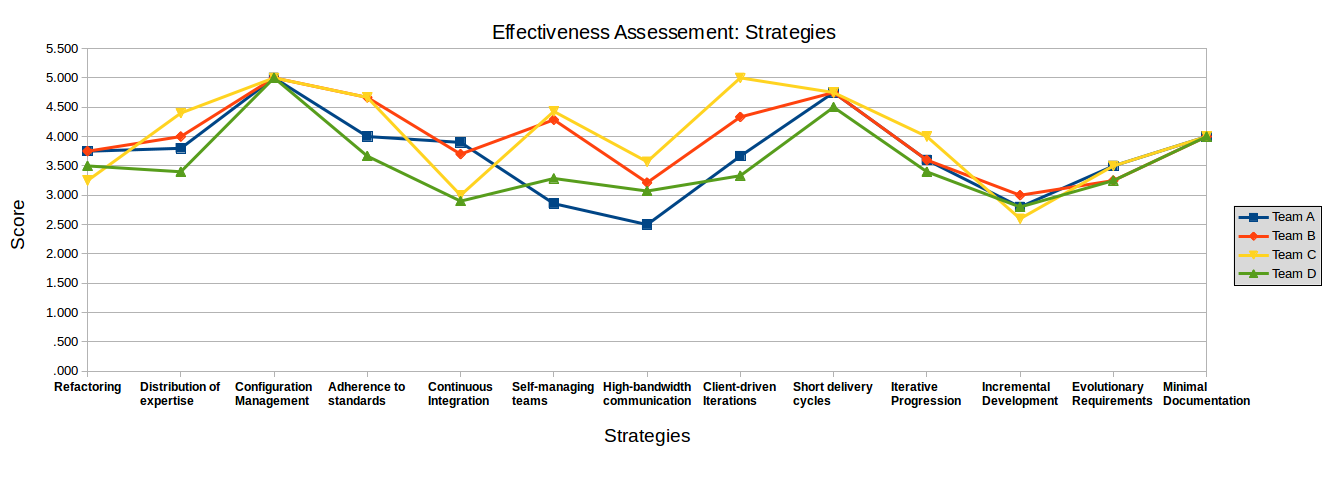
\includegraphics[scale=0.55]{include/case_study/fig/team_effectiveness_strategies.png}}
\caption{Effectiveness - Strategies level} 
\label{fig:team_effectiveness_strategies}
\end{figure}

\begin{figure}[H]
\centerline{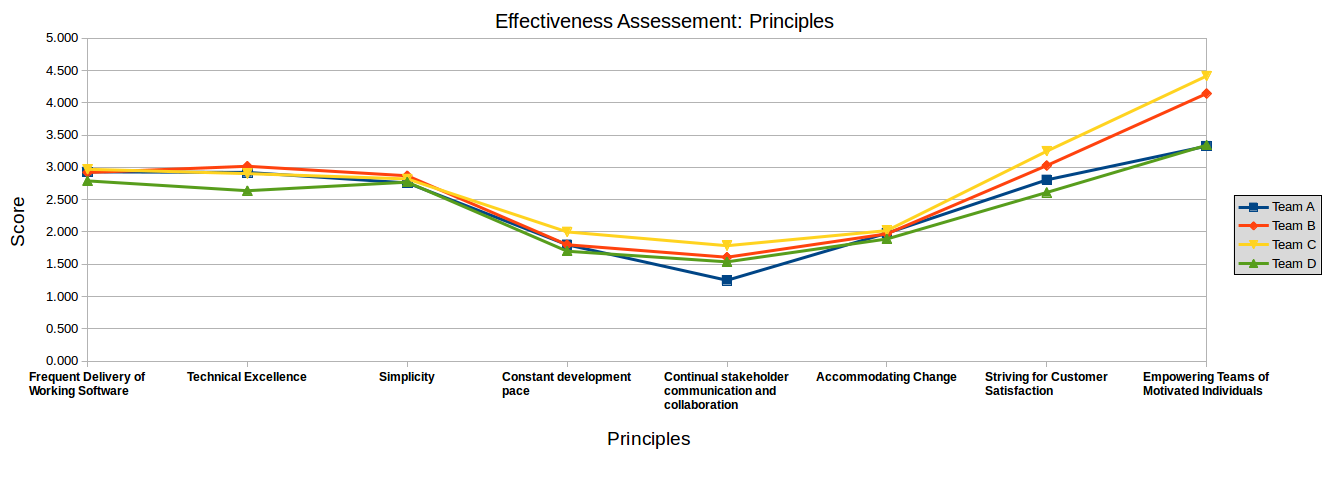
\includegraphics[scale=0.55]{include/case_study/fig/team_effectiveness_principles.png}}
\caption{Effectiveness - Principles level} 
\label{fig:team_effectiveness_principles}
\end{figure}

\begin{figure}[H]
\centerline{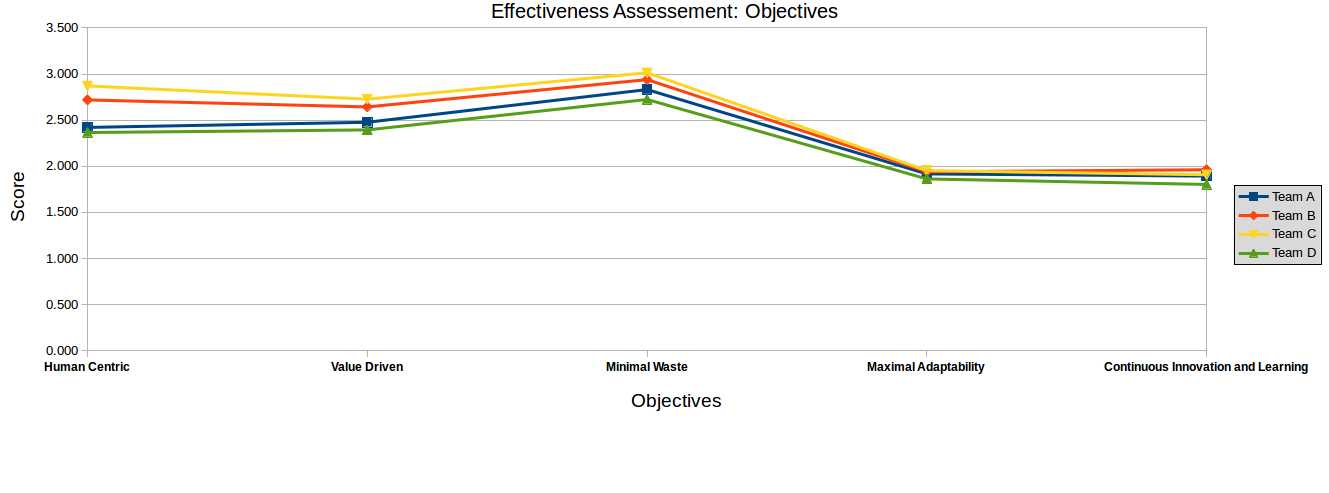
\includegraphics[scale=0.55]{include/case_study/fig/team_effectiveness_objectives.png}}
\caption{Effectiveness - Objectives level} 
\label{fig:team_effectiveness_objectives}
\end{figure}


\subsection{Results Verification}

\section{Perceptive Agile Measurement}
For assessing the agility by using the Perceptive Agile Measurement (PAM) tool, the teams were asked to answer on the survey seen in the~\nameref{sec:pam} Appendix. The answers were on a Likert scale 1-7.

\subsubsection{Team A Assessement}
\begin{tabular}{| p{3cm} | }
\hline
\textbf{Score:} value \\ \hline
\end{tabular}

\subsubsection{Team B Assessement}
\begin{tabular}{| p{3cm} | }
\hline
\textbf{Score:} value \\ \hline
\end{tabular}

\subsubsection{Team C Assessement}
\begin{tabular}{| p{3cm} | }
\hline
\textbf{Score:} value \\ \hline
\end{tabular}

\subsubsection{Team D Assessement}
\begin{tabular}{| p{3cm} | }
\hline
\textbf{Score:} value \\ \hline
\end{tabular}

\subsection{Results Verification}



\section{Team Agility Assessment}
\subsection{Results Verification}
~\nameref{sec:team_agility_assessment}

\section{Thoughtworks}
\subsection{Results Verification}

%\section{Tools Correlation}




\subsection{OPS}
Figure~\ref{objectives_principles_strategies}
\subsection{PAM}
\subsection{Leffingwell}
\section{Discussion}
